\subsection{Type checking}
\begin{figure}
\scriptsize{
\medskip
%%%%%%%%%%%%%%%%%%%%
$
\inferrule
{
}
{
\lins;\RefinementAny;\ABlockAny \vdash \skipstmt : \lins
}
\;(\textsc{Skip})
$
\medskip
%%%%%%%%%%%%%%%%%%%%
$
\inferrule
{
}
{
\lins;\RefinementAny;\ABlockOutside \vdash \assert{\locExpr} : \lins
}
\;(\textsc{Assert})
$
\medskip
%%%%%%%%%%%%%%%%%%%%
$
\inferrule
{
\lins_y \subseteq \lins
}
{
\lins;\RefinementAny;\ABlockOutside \vdash \yield{e,\lins_y} : \lins
}
\;(\textsc{Yield})
$
\medskip
%%%%%%%%%%%%%%%%%%%%
$
\inferrule
{
\ProcLins(A) = (\lins,\lins')
}
{
\lins;\RefinementAny;\ABlockInside \vdash \call{A} : \lins'
}
\;(\textsc{Atomic})
$
\medskip
%%%%%%%%%%%%%%%%%%%%
$
\inferrule
{
\ProcLins(P) = (\lins,\lins') \\
\RefinementAny = \RefinementInside \Longrightarrow P \in \dom(\refines)
}
{
\lins;\RefinementAny;\ABlockOutside \vdash \call{P} : \lins'
}
\;(\textsc{Proc})
$
\medskip
%%%%%%%%%%%%%%%%%%%%
$
\inferrule
{
\lins_G \subseteq \Globals \\
\lins \cup \lins_P \cup \lins_P' \subseteq \ThreadLocals \\
\ProcLins(P) = ((\lins_G,\lins_P),(\lins_G,\lins_P')) \\
\RefinementAny = \RefinementInside \Longrightarrow P \in \dom(\refines)
}
{
\lins_G,\lins,\lins_P;\RefinementAny;\ABlockOutside \vdash \async{P} : \lins_G,\lins
}
\;(\textsc{Async})
$
\medskip
%%%%%%%%%%%%%%%%%%%%
$
\inferrule
{
\lins;\RefinementAny;\ABlockInside \vdash \stmt : \lins' \\
\lins_a \subseteq \lins
}
{
\lins;\RefinementAny;\ABlockOutside \vdash \ablock{e,\lins_a}{\stmt} : \lins'
}
\;(\textsc{Ablock})
$
\medskip
%%%%%%%%%%%%%%%%%%%%
$
\inferrule
{
\lins;\RefinementAny;\ABlockAny \vdash \StmtStack : \lins'
}
{
\lins;\RefinementAny;\ABlockAny \vdash (\varsL,\StmtStack) : \lins'
}
\;(\textsc{StackFrame})
$
\medskip
%%%%%%%%%%%%%%%%%%%%
$
\inferrule
{
\lins;\RefinementAny;\ABlockAny \vdash \StmtStack : \lins' \\
\lins';\RefinementAny;\ABlockAny \vdash \stmt : \lins''
}
{
\lins;\RefinementAny;\ABlockAny \vdash \StmtStack;\stmt : \lins''
}
\;(\textsc{Seq})
$
\medskip
%%%%%%%%%%%%%%%%%%%%
$
\inferrule
{
\lins;\RefinementAny;\ABlockAny \vdash s_1 : \lins' \\
\lins;\RefinementAny;\ABlockAny \vdash s_2 : \lins'
}
{
\lins;\RefinementAny;\ABlockAny \vdash \ite{\locExpr}{s_1}{s_2} : \lins'
}
\;(\textsc{Ite})
$
\medskip
%%%%%%%%%%%%%%%%%%%%
$
\inferrule
{
\lins;\RefinementAny;\ABlockAny \vdash s : \lins
}
{
\lins;\RefinementAny;\ABlockAny \vdash \while{e}{\locExpr}{s} : \lins
}
\;(\textsc{While})
$
\medskip
%%%%%%%%%%%%%%%%%%%%
$
\inferrule
{
\ProcLins(P) = (\lins,\lins') \\
\RefinementAny = \RefinementInside \Longleftrightarrow P \in \dom(\refines) \\
\lins;\RefinementAny;\ABlockOutside \vdash \bodies(P) : \lins'
}
{
\vdash P
}
\;(\textsc{Procedure})
$
\medskip
%%%%%%%%%%%%%%%%%%%%
$
\inferrule
{
\ProcLins(A) = (\lins,\lins') \\
\lins \cap \Globals = \lins' \cap \Globals \\
\actions(A) = (\rho, \alpha, m) \\
m \in \{B, L\} \Longrightarrow \forall \sigma \in \rho. \exists \sigma'. (\sigma, \sigma') \in \alpha \\
A \in \mathit{range}(\refines) \Longrightarrow \accessVars(\rho) \subseteq \Locals \\
A \in \mathit{range}(\refines) \Longrightarrow \alpha = ((\exists \Locals,\Locals'.\alpha) \wedge \mathit{\Same(\Locals,\Locals')}) \\
\forall (\sigma,\sigma') \in \alpha.
  \biguplus\{lv(\sigma'(x)) \mid x \in \lins'\} \subseteq
  \biguplus\{lv(\sigma(x)) \mid x \in \lins\}
}
{
\vdash A
}
\;(\textsc{Action})
$
\medskip
%%%%%%%%%%%%%%%%%%%%
$
\inferrule
{
T = (\varsTL, (\varsL, \StmtStack)) \\
\lins;\RefinementOutside;\ABlockOutside \vdash \StmtStack : \lins'
}
{
\lins \vdash T
}
\;(\textsc{Thread})
$
\medskip
%%%%%%%%%%%%%%%%%%%%
$
\inferrule
{
\forall P \in \ProcName. \vdash P \\
\forall A \in \ActionName. \vdash A \\
\lins = \lins_G,\lins_1,\ldots,\lins_n  \\
\lins_G \subseteq \Globals \\
\forall 1 \le i \le n. (\lins_G,\lins_i \vdash T_i) \\
\forall 1 \le i \le n. (\lins_i \subseteq \ThreadLocals) \\
\forall 1 \le i \le n. (T_i = (\varsTL_i, \ldots)) \\
\biguplus\{lv(\varsG(x)) \mid x \in \lins_G\} \uplus
  \biguplus\{lv(\varsTL_i(x)) \mid 1 \le i \le n, x \in \lins_i\} \subseteq \linsmax
}
{
\vdash (\bodies, \actions, \specs, \refines, \ProcLins, \lins, \varsG, T_1 \ldots T_n)
}
\;(\textsc{Program})
$
\medskip
%%%%%%%%%%%%%%%%%%%%
}
\caption{Type checking rules}
\label{fig:type-checking}
\end{figure}

\subsection{Safety}
\begin{figure}
\scriptsize{
\medskip
%%%%%%%%%%%%%%%%%%%%
$
\inferrule
{
}
{\RefinementAny;\{\} \jp \FH{\phi}{\skipstmt}{\phi}}
\;(\textsc{Skip})
$
\medskip
%%%%%%%%%%%%%%%%%%%%
$
\inferrule
{
}
{\RefinementOutside;\{\} \jp \FH{\phi}{\assert{\locExpr}}{\phi}}
\;(\textsc{Assert1})
$
\medskip
%%%%%%%%%%%%%%%%%%%%
$
\inferrule
{
}
{\RefinementInside;\{\} \jp \FH{\phi \wedge \locExpr}{\assert{\locExpr}}{\phi}}
\;(\textsc{Assert2})
$
\medskip
%%%%%%%%%%%%%%%%%%%%
$
\inferrule
{
}
{\RefinementAny;\{\} \jp \FH{e}{\yield{e,\lins}}{e}}
\;(\textsc{Yield})
$
\medskip
~\\
%%%%%%%%%%%%%%%%%%%%
$
\inferrule
{
\actions(A) = (\rho, \alpha, m) \\ 
\mods \subseteq \ThreadLocals \\
\alpha \Rightarrow \Havoc(\Globals \cup \mods \cup \Locals) \\
\phi \Rightarrow \rho \\ 
\Unsat{\phi \circ \alpha \circ \neg \psi} \\
}
{\RefinementAny;\mods \jp \FH{\phi}{\call{A}}{\psi}}
\;(\textsc{Atomic})
$
\medskip
%%%%%%%%%%%%%%%%%%%%
$
\inferrule
{
\specs(P) = (\phi, \mods, \psi) \\ P \not \in \dom(\refines)
}
{\RefinementAny;\mods \jp \FH{\phi}{\call{P}}{\psi}}
\;(\textsc{Proc1})
$
\medskip
%%%%%%%%%%%%%%%%%%%%
$
\inferrule
{
\specs(P) = (\phi, \mods, \psi) \\ P \in \dom(\refines) \\\\ \RefinementAny;\mods \jp \FH{\phi}{\call{\refines(P)}}{\psi}
}
{\RefinementAny;\mods \jp \FH{\phi}{\call{P}}{\psi}}
\;(\textsc{Proc2})
$
\medskip
%%%%%%%%%%%%%%%%%%%%
$
\inferrule
{
\specs(P) = (\phi, \mods, \psi)
}
{\RefinementAny;\{\} \jp \FH{\rho \wedge \phi}{\async{P}}{\rho}}
\;(\textsc{Async})
$
\medskip
~\\
%%%%%%%%%%%%%%%%%%%%
$
\inferrule
{
\RefinementAny;\mods \jp \FH{\phi_1 \wedge e}{s}{\phi_2}
}
{\RefinementAny;\mods \jp \FH{\phi_1 \wedge e}{\ablock{e,\lins}{s}}{\phi_2}}
\;(\textsc{Ablock})
$
\medskip
%%%%%%%%%%%%%%%%%%%%
$
\inferrule
{
\RefinementAny;\mods_1 \jp \FH{\phi_1}{\StmtStack}{\phi_2} \\ \RefinementAny;\mods_2 \jp \FH{\phi_2}{s}{\phi_3}
}
{\RefinementAny;\mods_1 \cup \mods_2 \jp \FH{\phi_1}{\StmtStack;s}{\phi_3}}
\;(\textsc{Seq})
$
\medskip
%%%%%%%%%%%%%%%%%%%%
$
\inferrule
{
\RefinementAny;\mods_1 \jp \FH{e \wedge \phi_1}{s_1}{\phi_2} \\ \RefinementAny;\mods_2 \jp \FH{\neg e \wedge \phi_1}{s_2}{\phi_2}
}
{\RefinementAny;\mods_1 \cup \mods_2 \jp \FH{\phi_1}{\ite{\locExpr}{s_1}{s_2}}{\phi_2}}
\;(\textsc{Ite})
$
\medskip
%%%%%%%%%%%%%%%%%%%%
$
\inferrule
{
\RefinementAny;\mods \jp \FH{e \wedge \locExpr}{s}{e}
}
{\RefinementAny;\mods \jp \FH{e}{\while{e}{\locExpr}{s}}{e \wedge \neg \locExpr}}
\;(\textsc{While})
$
\medskip
%%%%%%%%%%%%%%%%%%%%
$
\inferrule
{
\RefinementAny;\mods \jp \phi \Rightarrow \phi' \\ \RefinementAny;\mods \jp \FH{\phi'}{\StmtStack}{\psi'} \\ \psi' \Rightarrow \psi
}
{\RefinementAny;\mods \jp \FH{\phi}{\StmtStack}{\psi}}
\;(\textsc{Weaken})
$
\medskip
%%%%%%%%%%%%%%%%%%%%
$
\inferrule
{
\RefinementAny;\mods \jp \FH{\phi}{\StmtStack}{\psi} \\ \accessVars(\rho) \cap \mods = \{\}
}
{\RefinementAny;\mods \jp \FH{\rho \wedge \phi}{\StmtStack}{\rho \wedge \psi}}
\;(\textsc{Frame})
$
\medskip
%%%%%%%%%%%%%%%%%%%%
$
\inferrule
{
\specs(P) = (\phi, \mods, \psi) \\
\RefinementAny = \RefinementInside \Longleftrightarrow P \in \dom(\refines) \\\\
\RefinementAny;\mods' \jp \FH{\phi}{\bodies(P)}{\psi} \\
\mods' \subseteq \mods
}
{
\jp P
}
\;(\textsc{Procedure})
$
\medskip
%%%%%%%%%%%%%%%%%%%%
$
\inferrule
{
\RefinementAny;\mods \jp \FH{\phi'}{\StmtStack}{\psi} \\ 
(\accessVars(\phi) \cup \accessVars(\psi)) \cap \Locals = \{\} \\
\forall G, \varsTL.\ \phi(G,\varsTL) \Rightarrow \phi'(G, \varsTL,\varsL)
}
{
\RefinementAny;\mods \jp \FH{\phi}{(\varsL,\StmtStack)}{\psi}
}
\;(\textsc{StackFrame})
$
\medskip
%%%%%%%%%%%%%%%%%%%%
$
\inferrule
{
T = (\varsTL, (\varsL, \StmtStack)) \\
G\!\cdot\!\varsTL\!\cdot\!\varsL \jp \phi \rightarrow \true \\\\
\RefinementOutside;\mods \jp \FH{\phi}{(\varsL,\StmtStack)}{\true}
}
{
G \jp T
}
\;(\textsc{Thread})
$
\medskip
%%%%%%%%%%%%%%%%%%%%
$
\inferrule
{
\forall P \in \ProcName.\ \jp P \\
\forall 1 \le i \le n.\ G \jp T_i
}
{
\jp (\bodies, \actions, \specs, \refines, \varsG, T_1 \ldots T_n)
}
\;(\textsc{Program})
$
\medskip
%%%%%%%%%%%%%%%%%%%%
}
\caption{Sequential rules for partial correctness}
\label{fig:sequential-correctness}
\end{figure}

{\bf Non-interference.}
Let $\Yields$ be the set of yield predicates, preconditions, and postconditions in the program.
Let $\Ablocks$ be the set of atomic blocks in the program except those inside the bodies of procedures
in $\dom(\refines)$.
Let $\FV \subseteq \VarName \setminus \Var$ be a set of fresh variables and $\Lambda$ be a one-one 
substitution function from $\ThreadLocals \cup \Locals$ to $\FV$.
Let $\Lambda(\phi)$ represent the result of applying $\Lambda$ to the expression $\phi$.
For each predicate ($\phi,\lins_y) \in \Yields$
and for each atomic block $\ablock{e,\lins_a}{s} \in \Ablocks$, we prove the following judgment:
\[
\FH{\Lambda(\phi) \wedge e \wedge
  \{lv(\Lambda(x)) \mid x \in \lins_y\} \uplus
  \{lv(x) \mid x \in \lins_a\} \subseteq \linsmax
}{s}{\Lambda(\phi)}
\]
For each predicate $\phi \in \Yields$ and for each $P \in \dom(\refines)$ such that
$\actions(\refines(P)) = (\rho, \alpha, m)$, we prove the following to be unsatisfiable:
\[
\Lambda(\phi) \circ \rho \circ \alpha \circ \neg\Lambda(\phi)
\]

\subsection{Refinement}
\begin{figure}
\scriptsize{
\medskip
%%%%%%%%%%%%%%%%%%%%
$
\inferrule
{
}
{P \jr \skipstmt : \epsilon}
\;(\textsc{Skip})
$
\medskip
%%%%%%%%%%%%%%%%%%%%
$
\inferrule
{
}
{P \jr \assert{\locExpr} : \epsilon}
\;(\textsc{Assert})
$
\medskip
%%%%%%%%%%%%%%%%%%%%
$
\inferrule
{
}
{P \jr \yield{e,\lins} : \epsilon}
\;(\textsc{Yield})
$
\medskip
%%%%%%%%%%%%%%%%%%%%
$
\inferrule
{
\actions(\refines(P')) = (\rho',\alpha',m) \\\\ \rho' \circ \alpha' \Rightarrow \Havoc(\{\})
}
{P \jr \call{P'} : \epsilon}
\;(\textsc{Call-Loop})
$
\medskip
%%%%%%%%%%%%%%%%%%%%
$
\inferrule
{
\actions(\refines(P)) = (\rho,\alpha,m) \\ \actions(\refines(P')) = (\rho',\alpha',m) \\\\ \rho' \circ \alpha' \Rightarrow \exists \Locals, \Locals'.\ \alpha
}
{P \jr \call{P'} : N}
\;(\textsc{Call-Action})
$
\medskip
%%%%%%%%%%%%%%%%%%%%
$
\inferrule
{
\actions(\refines(P')) = (\rho',\alpha',m) \\ \rho' \circ \alpha' \Rightarrow \Havoc(\{\})
}
{P \jr \async{P'} : \epsilon}
\;(\textsc{Async})
$
\medskip
%%%%%%%%%%%%%%%%%%%%
$
\inferrule
{
s \preceq \mathit{old}(e) \Rightarrow \Havoc(L)
}
{P \jr \ablock{e,\lins}{s} : \epsilon}
\;(\textsc{Ablock-Loop})
$
\medskip
%%%%%%%%%%%%%%%%%%%%
$
\inferrule
{
\actions(\refines(P)) = (\rho,\alpha,m) \\ s \preceq \mathit{old}(e) \Rightarrow  \exists \Locals, \Locals'.\ \alpha
}
{P \jr \ablock{e,\lins}{s} : N}
\;(\textsc{Ablock-Action})
$
\medskip
%%%%%%%%%%%%%%%%%%%%
$
\inferrule
{
P \jr s_1 : \re_1 \\ P \jr s_2 : \re_2
}
{P \jr s_1;s_2 : \re_1\cdot\re_2}
\;(\textsc{Seq})
$
\medskip
%%%%%%%%%%%%%%%%%%%%
$
\inferrule
{
P \jr s_1 : \re_1 \\ P \jr s_2 : \re_2
}
{P \jr \ite{\locExpr}{s_1}{s_2} : \re_1+\re_2}
\;(\textsc{Ite})
$
\medskip
%%%%%%%%%%%%%%%%%%%%
$
\inferrule
{
P \jr s : \re
}
{P \jr \while{e}{\locExpr}{s} : \re^*}
\;(\textsc{While})
$
\medskip
%%%%%%%%%%%%%%%%%%%%
$
\inferrule
{
\forall P \in \dom(\refines).\ \bodies(P) \jr \{N\}
}
{
\jr (\bodies, \actions, \specs, \refines, \varsG, T_1 \ldots T_n)
}
\;(\textsc{Program})
$
\medskip
%%%%%%%%%%%%%%%%%%%%
}
\caption{Refinement rules}
\label{fig:refinement}
\end{figure}

\begin{figure}
\scriptsize{
\medskip
%%%%%%%%%%%%%%%%%%%%
$
\inferrule
{
}
{\skipstmt \preceq \Havoc(\{\})}
\;(\textsc{Skip})
$
\medskip
%%%%%%%%%%%%%%%%%%%%
$
\inferrule
{
}
{\assert{\locExpr} \preceq \Havoc(\{\})}
\;(\textsc{Assert})
$
\medskip
%%%%%%%%%%%%%%%%%%%%
$
\inferrule
{
}
{\yield{e,\lins} \preceq \false}
\;(\textsc{Yield})
$
\medskip
%%%%%%%%%%%%%%%%%%%%
$
\inferrule
{
\actions(A) = (\rho, \alpha, m) 
}
{\call{A} \preceq \alpha}
\;(\textsc{Atomic})
$
\medskip
%%%%%%%%%%%%%%%%%%%%
$
\inferrule
{
}
{\call{P} \preceq \false}
\;(\textsc{Call})
$
\medskip
%%%%%%%%%%%%%%%%%%%%
$
\inferrule
{
}
{\async{P} \preceq \Havoc(\{\})}
\;(\textsc{Async})
$
\medskip
%%%%%%%%%%%%%%%%%%%%
$
\inferrule
{
s \preceq \alpha
}
{\ablock{e,\lins}{s} \preceq \alpha}
\;(\textsc{Ablock})
$
\medskip
%%%%%%%%%%%%%%%%%%%%
$
\inferrule
{
s_1 \preceq \alpha_1 \\ s_2 \preceq \alpha_2
}
{s_1;s_2 \preceq \alpha_1 \circ \alpha_2}
\;(\textsc{Seq})
$
\medskip
%%%%%%%%%%%%%%%%%%%%
$
\inferrule
{
s_1 \preceq \alpha_1 \\ s_2 \preceq \alpha_2
}
{\ite{\locExpr}{s_1}{s_2} \preceq (\locExpr \circ \alpha_1) \vee (\neg \locExpr \circ \alpha_2)}
\;(\textsc{Ite})
$
\medskip
%%%%%%%%%%%%%%%%%%%%
$
\inferrule
{
s \preceq \beta \\ \neg \locExpr \circ \Havoc(\{\}) \Rightarrow \alpha \\ \beta \circ \alpha \Rightarrow \alpha 
}
{\while{e,\alpha}{\locExpr}{s} \preceq e \circ \alpha \circ \neg \locExpr}
\;(\textsc{While})
$
\medskip
%%%%%%%%%%%%%%%%%%%%
$
\inferrule
{
s \preceq \alpha \\ \alpha \Rightarrow \alpha'
}
{s \preceq \alpha'}
\;(\textsc{Weaken})
$
\medskip
}
\caption{Abstracting statements by actions}
\label{fig:statement-to-action}
\end{figure}

\subsection{Yield sufficiency}

{\bf Commutativity.}
Let $\FV_1,\FV_2 \subseteq \VarName \setminus \Var$ be two sets of disjoint fresh variables.
Let $\Lambda_1$ and $\Lambda_2$ be one-one 
substitution functions from $\ThreadLocals \cup \Locals$ to $\FV_1$ and $\FV_2$ respectively.
For all $A_1,A_2 \in \ActionName$ such that $\actions(A_1) = (\rho_1,\alpha_1,m_1)$ and $\actions(A_2) = (\rho_2,\alpha_2,m_2)$,
if $m_1 \in \{B,R\}$ or $m_2 \in \{B,L\}$ then prove the following valid:
\[
\begin{array}{l}
(\Lambda_1(\rho_1) \wedge \Lambda_2(\rho_2)) \circ (\Lambda_1(\alpha_1) \wedge \Same(\FV_2)) \circ (\Lambda_1(\alpha_2) \wedge \Same(\FV_1)) \\ 
\Rightarrow (\Lambda_1(\alpha_2) \wedge \Same(\FV_1)) \circ (\Lambda_1(\alpha_1) \wedge \Same(\FV_2))
\end{array}
\]
For all $A_1,A_2 \in \ActionName$ such that $\actions(A_1) = (\rho_1,\alpha_1,m_1)$ and $\actions(A_2) = (\rho_2,\alpha_2,m_2)$,
if $m_1 \in \{B,R\}$ then prove the following unsatisfiable:
\[
\Lambda_1(\rho_1) \circ (\Lambda_2(\rho_2) \circ \Lambda_2(\alpha_2)) \circ \neg \Lambda_1(\rho_1)
\]
For all $A_1,A_2 \in \ActionName$ such that $\actions(A_1) = (\rho_1,\alpha_1,m_1)$ and $\actions(A_2) = (\rho_2,\alpha_2,m_2)$,
if $m_1 \in \{B,L\}$ then prove the following unsatisfiable:
\[
\neg \Lambda_1(\rho_1) \circ (\Lambda_2(\rho_2) \circ \Lambda_2(\alpha_2)) \circ \Lambda_1(\rho_1)
\]

\begin{figure}
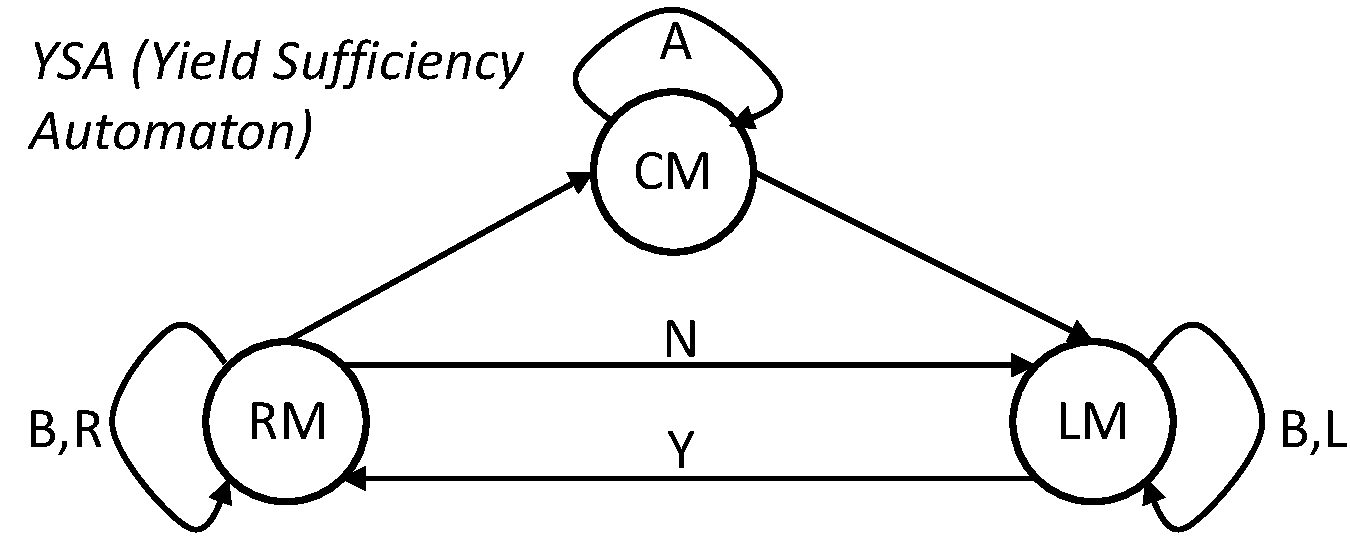
\includegraphics[scale=0.35]{YieldTypeCheckingAutomaton.pdf}
\caption{Specification for yield sufficiency}
\label{fig:YieldTypeCheckingAutomaton}
\end{figure}

\begin{figure}
\scriptsize{
\medskip
%%%%%%%%%%%%%%%%%%%%
$
\inferrule
{
}
{\jy \skipstmt : (x, x)}
\;(\textsc{Skip})
$
\medskip
%%%%%%%%%%%%%%%%%%%%
$
\inferrule
{
}
{\jy \assert{\locExpr} : (x, x)}
\;(\textsc{Assert})
$
\medskip
%%%%%%%%%%%%%%%%%%%%
$
\inferrule
{
}
{\jy \yield{e,\lins} : (x, \RM)}
\;(\textsc{Yield})
$
\medskip
~\\
%%%%%%%%%%%%%%%%%%%%
$
\inferrule
{
P \in \dom(\refines) \\ \actions(\refines(P)) = (\rho, \alpha, B)
}
{\jy \call{P} : (x, x)}
\;(\textsc{CallBothMover})
$
\medskip
%%%%%%%%%%%%%%%%%%%%
$
\inferrule
{
P \in \dom(\refines) \\ \actions(\refines(P)) = (\rho, \alpha, R)
}
{\jy \call{P} : (\RM, \RM)}
\;(\textsc{CallRightMover})
$
\medskip
%%%%%%%%%%%%%%%%%%%%
$
\inferrule
{
P \in \dom(\refines) \\ \actions(\refines(P)) = (\rho, \alpha, L)
}
{\jy \call{P} : (x, \LM)}
\;(\textsc{CallLeftMover})
$
\medskip
%%%%%%%%%%%%%%%%%%%%
$
\inferrule
{
P \in \dom(\refines) \\ \actions(\refines(P)) = (\rho, \alpha, N)
}
{\jy \call{P} : (\RM, \LM)}
\;(\textsc{CallNonMover})
$
\medskip
%%%%%%%%%%%%%%%%%%%%
$
\inferrule
{
P \not \in \dom(\refines)
}
{\jy \call{P} : (x, \RM)}
\;(\textsc{CallYield})
$
\medskip
%%%%%%%%%%%%%%%%%%%%
$
\inferrule
{
}
{\jy \async{P} : (x, \LM)}
\;(\textsc{Async})
$
\medskip
%%%%%%%%%%%%%%%%%%%%
$
\inferrule
{
x \in \{\RM,\CM\}
}
{\jy \ablock{e,\lins}{s} : (x, \CM)}
\;(\textsc{Ablock})
$
\medskip
%%%%%%%%%%%%%%%%%%%%
$
\inferrule
{
\jy \StmtStack : (x, y) \\ \jy s : (y, z)
}
{\jy \StmtStack;s : (x, z)}
\;(\textsc{Seq})
$
\medskip
%%%%%%%%%%%%%%%%%%%%
$
\inferrule
{
\jy s_1 : (x, y) \\ \jy s_2 : (x, y)
}
{\jy \ite{\locExpr}{s_1}{s_2} : (x, y)}
\;(\textsc{Ite})
$
\medskip
%%%%%%%%%%%%%%%%%%%%
$
\inferrule
{
\jy s : (x, x)
}
{\jy \while{e}{\locExpr}{s} : (x, x)}
\;(\textsc{While})
$
\medskip
%%%%%%%%%%%%%%%%%%%%
$
\inferrule
{
\jy \bodies(P) : (x, y)
}
{
\jy P
}
\;(\textsc{Procedure})
$
\medskip
%%%%%%%%%%%%%%%%%%%%
$
\inferrule
{
\jy \StmtStack : (x,y)
}
{
\jy (\varsL,\StmtStack) : (x,y)
}
\;(\textsc{StackFrame})
$
\medskip
%%%%%%%%%%%%%%%%%%%%
$
\inferrule
{
T = (\varsTL, (\varsL, \StmtStack)) \\
\jy (\varsL, \StmtStack) : (x, y)
}
{
\jy T
}
\;(\textsc{Thread})
$
\medskip
%%%%%%%%%%%%%%%%%%%%
$
\inferrule
{
\forall P \in \ProcName \setminus \dom(\refines).\ \jy P \\
\forall 1 \le i \le n.\ \jy T_i
}
{
\jy (\bodies, \actions, \specs, \refines, \varsG, T_1 \ldots T_n)
}
\;(\textsc{Program})
$
\medskip
%%%%%%%%%%%%%%%%%%%%
}
\caption{Yield sufficiency rules}
\label{fig:yield-sufficiency}
\end{figure}

\subsection{Soundness}

\begin{theorem}
Let $\Prog$ and $\Prog'$ be two programs such that the following conditions are satisfied:
\begin{enumerate}
\item
$\vdash \Prog$ and $\vdash \Prog'$ and $\Prog$ is abstracted by $\Prog'$.
\item 
All finite executions of $\Prog'$ are safe.
\item
All infinite executions of $\Prog'$ are responsive.
\item
The program $\Prog$ is commutativity-safe.
\item
The program $\Prog$ is interference-free.
\item
$\jp Prog$, $\jr Prog$, and $\jy Prog$.
\end{enumerate}
Then all finite executions of $\Prog'$ are safe.
\end{theorem}

\subsection{Responsiveness}

\[
\inferrule
{
\FH{e \wedge \locExpr}{s}{e} \\ e \wedge \locExpr \Rightarrow f \geq 0 \\ s \preceq (old(e \wedge \locExpr) \Rightarrow \mathit{old}(f) > f)
}
{\FH{e}{\while{e,\alpha,f}{\locExpr}{s}}{e \wedge \neg \locExpr}}
\;(\textsc{While})
\]

